\section{VoiceFilter-Lite}
VoiceFilter-Lite \cite{wang2020voicefilterlite} is one of the future versions of VoiceFilter \cite{wang2019voicefilter}, which can be summarized as a single channel source separation model for a target speaker, which is mainly a part of on-device streaming ASR (Automatic Speech Recognition), where takes filter-banks as inputs and outputs, and it is a quantized 8-bit model to reduce its size.

\subsection{Model Architecture}

\begin{figure}
  \centering
  \begin{subfigure}{.3\textwidth}
    \centering
    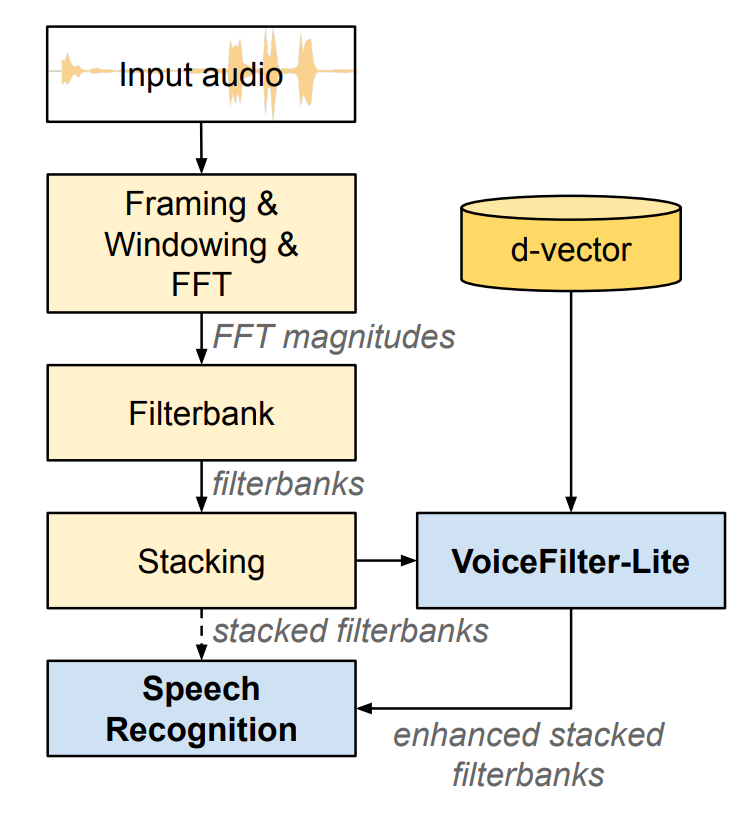
\includegraphics[width=.9\linewidth]{images/related_work/voicefilter-lite/voicefilter-lite-asr.png}
    \caption{}
    \label{fig:voicefilter-lite-asr}
  \end{subfigure}%
  \begin{subfigure}{.7\textwidth}
    \centering
    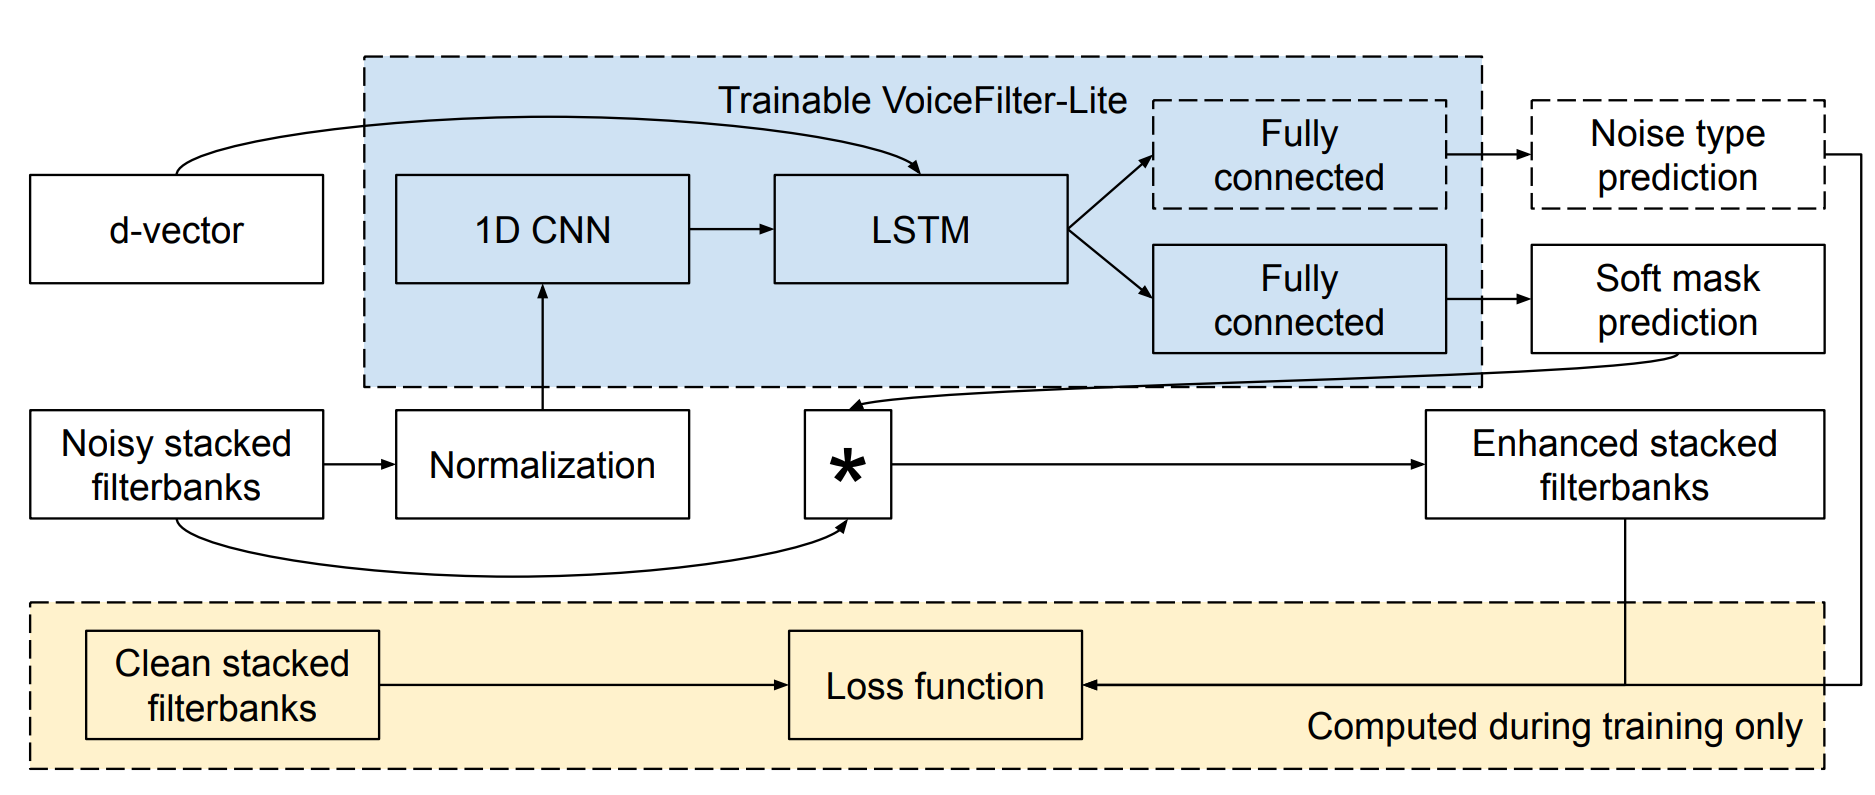
\includegraphics[width=.9\linewidth]{images/related_work/voicefilter-lite/voicefilter-lite-arch.png}
    \caption{}
    \label{fig:voicefilter-lite-model}
  \end{subfigure}
  \caption{VoiceFilter-Lite architecture, assuming using stacked filterbank energies as inputs and outputs. (a) Integration with ASR. The dashed arrow indicates the original connection without VoiceFilter-Lite. (b) Neural network topology of the VoiceFilter-Lite model.}
  \label{fig:voicefilter-lite}
\end{figure}

Figure \ref{fig:voicefilter-lite-asr} shows how the VoiceFilter-Lite can be integrated with the ASR System, while Figure \ref{fig:voicefilter-lite-model} shows the actual model topology of VoiceFilter-Lite where it is similar to the Original VoiceFilter but with a few differences to guarantee minimal latency:
\begin{itemize}
  \item Limited convolution layers to be 1D instead of 2D, where the kernels are now in the frequency dimension only.
  \item LSTM layers must be unidirectional and must take streaming inputs.
\end{itemize}
Since 1D-CNN is not as powerful as 2D-CNN, the model mainly consists of LSTM layers.

\subsubsection{Model Quantization}
The network parameters are stored in 32-bit floating point values in raw TensorFlow graphs, which are not well suited for on-device inference. The models are serialized to the FlatBuffer TensorFlow Lite format and use dynamic range quantization to quantize the network parameters to 8-bit integers. This allows us to better utilize the improved hardware instructions for integer arithmetic and drastically lower the cost of memory.

\subsection{Experimental Setup}
Since the goal of the VoiceFilter-Lite model is to enhance on-device ASR, our statistic of choice is the Word Error Rate (WER). In particular, they were concerned about the WER in different noise situations both before and after using VoiceFilter-Lite. Given the emphasis on speech recognition and the fact that the VoiceFilter-Lite model does not reconstruct any waveform from the enhanced acoustic features, metrics like signal-to-noise ratio (SNR) or source-to-distortion ratio (SDR) that have been widely used for conventional source separation were not reported.

\subsubsection{Model and Data}
In the experiments, the VoiceFilter-Lite model has 3 LSTM layers, each with 512 nodes, and a final fully connected layer with sigmoid activation. If noise type prediction is enabled, it has another two feedforward layers, each with 64 nodes, and is trained with a hinge loss for binary classification. The training data consist of:
\begin{enumerate}
  \item The LibriSpeech \cite{librispeech} training set.
  \item A vendor collected a dataset of realistic speech queries.
\end{enumerate}
The study evaluates data using various noise sources and room configurations. The original non-modified data is referred to as "Clean", while the speech noise source is a distinct development set. The evaluations are conducted under two room conditions: "Additive" which adds noise waveforms to the clean waveform, and "Reverb" which generates 3 million convolutional room impulse responses (RIR) from a room simulator. The SNR is drawn from a uniform distribution from 1dB to 10dB for both additive and reverberant conditions.

\subsection{Conclusion}
VoiceFilter-Lite is a fast, tiny model that performs targeted voice separation in a streaming fashion for on-device ASR systems. It ensures ASR performance without affecting non-speech noise and reverberant room conditions. The model is trained with an asymmetric loss function and adaptive suppression strength at run-time. The 2.2 MB model has no WER degradation on clean and non-speech noise conditions while improving ASR performance on overlapped speech.